\documentclass[mathserif]{beamer}
\usetheme[secheader]{pecostalk}
\usepackage{amsmath}
\usepackage{subfigure}
\graphicspath{{figs/}}    
\newcommand{\Lo}{\,\mathcal{L}}
\newcommand{\Diff}[2] {\dfrac{\partial( #1)}{\partial #2}}
\newcommand{\ms}{\hat{u}}
\newcommand{\bv}[1]{\ensuremath{\mbox{\boldmath$ #1 $}}}
\newcommand{\pp}[2]{\frac{\partial #1}{\partial #2}}
\newcommand{\dd}[2]{\frac{d #1}{d #2}}
\newcommand{\DD}[2]{\frac{D #1}{D #2}}
\newcommand{\mm}{\mathbf{minmod}}
\def\etal{{\it et al~}}
\newcommand{\be}{\begin{eqnarray}}
\newcommand{\ee}{\end{eqnarray}}
\newcommand{\mbb}[1]{\mathbb{#1}} % math blackboard bold
\newcommand{\mrm}[1]{\mathrm{#1}} % math Roman
\newcommand{\mcal}[1]{\mathcal{#1}} % math blackboard bold
\newcommand{\mbf}[1]{\mathbf{#1}} % math bold face (for vectors)
\newcommand{\sbf}[1]{\boldsymbol{#1}} % bold face for symbols
\newcommand{\jump}[1]{\llbracket #1 \rrbracket} % jump operator
\newcommand{\avg}[1]{\{ #1 \}} % average operator
\newcommand{\rarrow}{\rightarrow}
\newcommand{\Rarrow}{\Rightarrow}
\newcommand{\LRarrow}{\Leftrightarrow}
\newcommand{\vvvert}{|\kern-1pt|\kern-1pt|}
\newcommand{\enorm}[1]{\vvvert #1 \vvvert}
\newcommand{\nutil}{\tilde{\nu}}
\newcommand{\myred}[1]{{\color{red} #1}}
\newcommand{\sa}{\nu_{\mathrm{sa}}}
\newcommand{\brho}{\bar{\rho}}
\newcommand{\tu}{\tilde{u}}
\newcommand{\tv}{\tilde{v}}
\newcommand{\tS}{\tilde{S}}
\newcommand{\tE}{\tilde{E}}
\newcommand{\bmu}{\bar{\mu}}
\newcommand{\hh}{\tilde{h}}
\newcommand{\bp}{\bar{p}}
\newcommand{\tsa}{\mathrm{sa}}

\definecolor{Purple}{rgb}{.8,0,.8}
\definecolor{Red}{rgb}{1,0,0}
\definecolor{DarkRed}{rgb}{.5,0,0}
\definecolor{Blue}{rgb}{0,0,1}
\definecolor{DarkCyan}{rgb}{0,.6,.6}
\definecolor{DarkGreen}{rgb}{0,.5,0}

\newcommand{\data}[1]{\texttt{\color{DarkRed}#1}}
\newcommand{\comment}[1]{\texttt{\color{Red}#1}}
\newcommand{\pdv}[2]{\frac{\partial #1}{\partial #2}}
\newcommand{\Reals}{{\ensuremath{\mathbb{R}}}}
\newcommand{\Complex}{{\ensuremath{\mathbb{C}}}}
\newcommand{\Duals}{{\ensuremath{\mathbb{D}}}}
\newcommand{\Hyperduals}{{\ensuremath{\mathbb{H}}}}
\newcommand{\type}[1]{\texttt{\color{DarkGreen}#1}}
\newcommand{\omission}{{\vspace{-.7em}.........\vspace{-.3em}}}
\newcommand{\var}[1]{\texttt{\color{Blue}#1}}
\newcommand{\func}[1]{\texttt{\color{DarkCyan}#1}}
\newcommand{\key}[1]{\texttt{\color{Purple}#1}}
\newcommand{\itemdone}{\item[{\color{pecos2}\Checkmark}]}
\newcommand{\checkm}{\color{pecos2}\Checkmark}

\date{June 30th, 2014}
\author[Nicholas Malaya]{Nicholas Malaya \\
$~$ \\
{\small
Center for Predictive Engineering and Computational Sciences (PECOS) \\
Institute for Computational Engineering and Sciences (ICES) \\
The University of Texas at Austin
}
}
\title[Software Verification Workshop]{Software Verification Workshop}

\begin{document}
\begin{frame}
  \begin{center}
    
\includegraphics[width=.8\linewidth]{grand_logo}\\
  \end{center}
  \titlepage
  \begin{flushright}
    
\includegraphics[scale=0.1]{asc_logo}\\
  \end{flushright}
\end{frame}

%===============================================================================
% goals of workshop
%===============================================================================
\begin{frame}[fragile]
  \frametitle{Workshop}
% This talk is online:
 % achtung! update me
  This talk is online:
\begin{verbatim}users.ices.utexas.edu/~nick/collaborate/lanl \end{verbatim}

  \begin{block}{Goals}
    \begin{itemize} 
    \item Walk you through the process of code verification
    \item Build/install MASA
    \item Do a grid-refinement study for solution verification
    \item Write some code to have a little fun - do something simple
      and use MASA
    \end{itemize}    
  \end{block}

\end{frame}

%===============================================================================
% refresher
%===============================================================================
\begin{frame}
  \frametitle{Problem: Solve 2D Laplacian using Finite-Differencing}
  \begin{columns}[c]
    \begin{column}{5cm}

      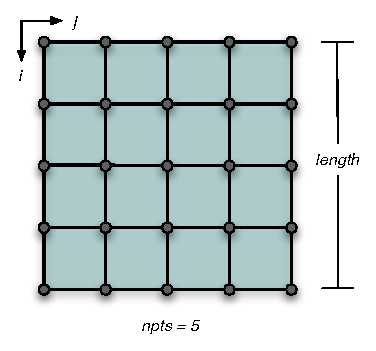
\includegraphics[width=1\linewidth]{domain}

    \end{column}
    
    \begin{column}{6.5cm}
      
      \begin{block}{Recall:}
        \begin{itemize} 

          \item Laplace's Equation in 2D:
          \begin{equation}
            \nonumber     
            \frac{\partial^2 \phi}{\partial x^2} + \frac{\partial^2 \phi}{\partial y^2} = 0
          \end{equation}

	  \item For the verification exercise, we will replace the RHS
	    above with a forcing function $f(x,y)$ that we get from
	    MASA
          \begin{equation}
            \nonumber     
            \frac{\partial^2 \phi}{\partial x^2} + \frac{\partial^2
	      \phi}{\partial y^2} = f(x,y)
	    \end{equation}
          
          % nick: not sure about this here, do we want to show mms?
          % seems less useful to remind them about the source term
%%           \item Our manufactured solution is:
%%           \begin{equation}
%%             \begin{split}
%%               \nonumber
%%               \phi(x,y) &= (\textcolor{blue}{Ly}-y)^2 (\textcolor{blue}{Ly}+y)^2 \\ 
%%               &+ (\textcolor{red}{Lx}-x)^2 (\textcolor{red}{Lx}+x)^2
%%             \end{split}
%%           \end{equation}          
%%           \item By default, \textcolor{blue}{Ly}$=0.82$ and \textcolor{red}{Lx}$=1.4$

        \end{itemize}    
      \end{block}
      
    \end{column}
  \end{columns}

%%   % karl: can you check that this is the differencing scheme you intended?
%%   Solve using forward difference:
%%   \begin{equation}
%%     \nonumber     
%%     \phi_i'' \approx \frac{\phi_{i+2} - 2\phi_{i+1} + \phi_{i}}{h^2} + O(h^2)
%%   \end{equation}
  
\end{frame}

 \begin{frame}
   \frametitle{Problem: Solve 2D Laplacian using Finite-Differencing}

   \begin{block}{Outline}
     \begin{itemize} 
     \item {\em Goal:} Write a program in C/C++, F90, python, or Matlab/Octave
       which solves the two-dimensional Laplacian on a square domain
     \item {\em Inputs}: 
       \begin{itemize}
	 \item \# of points in one direction ({\em npts})
	 \item the physical dimension of one side ({\em length})
       \end{itemize}
     \item {\em Output}: $l_2$ error between your numerical solution
       and an exact solution derived from a manufactured solution in
       MASA
       \begin{equation}
         \nonumber
         l_2 = \sqrt{ \frac{\sum_{i=1}^{\text{\tiny N}} (\phi_i-\phi_i^{\text{\tiny exact}})^2}N}
       \end{equation}
     \item {\em Runs}: Run your snazzy code for $\text{npts} =
       5,9,17,\text{and } 33$ and plot $l_2$ norm as a function of $1/h$ where
       $h=\text{length}/(\text{npts}-1)$
       
     \end{itemize}    
   \end{block}

 \end{frame}

\begin{frame}
  \frametitle{Finite-difference Scheme}
    \begin{block}{Method}
      \begin{itemize} 
	\item Let us use a simple FD approximation for the Laplacian
        \item Assume a constant spacing mesh for convenience
        \item Central-differencing 
	  \begin{equation}
	    \nonumber     
	    \nabla^{2}{\phi}_{i,j} \approx \frac{\phi_{i+1,j} -
	      2\phi_{i,j} + \phi_{i-1,j}}{h^2} + 
	    \frac{\phi_{i,j+1} -
	      2\phi_{i,j} + \phi_{i,j-1}}{h^2} + O(h^2)
	  \end{equation}
	  \item Use this formula to build the coefficient entries into
	    a linear system $Ax=b$.  
	  \item The size of the linear system is the number of solution
	    points. Since we are on a square domain,  $N = \text{npts}*\text{npts}$
      \end{itemize}
    \end{block}
\end{frame}

\begin{frame}
  \frametitle{Finite-difference Scheme}
    \begin{block}{Boundary Conditions}
      \begin{itemize} 
          \item The 5-point FD stencil is incomplete on the boundaries of
	    our square domain 
	  \item We need to apply constraints to matrix
	    $A$ to enforce the Dirchlet conditions on the boundaries
	  \item Simplest method to enforce BCs:
	    \begin{itemize} 
	      \item zero out all matrix entries on the
		row associated with boundary point, $\phi_i$
	    \item set the
	      diagonal $A(i,i)$ = 1.0
	      \item Set the RHS function to the
		desired solution $f_i = \phi_{\text{exact}}$
		\end{itemize}
      \end{itemize}
    \end{block}
\end{frame}

\begin{frame}[fragile]
  \frametitle{Finite-difference Scheme}
    \begin{block}{Boundary Conditions}
      \begin{itemize} 
          \item Let's look at form of system matrix $A^*$ after BCs have
	    been applied for $\text{npts}=3$ (note $A=\frac{1}{h^2}A^*$):
{\tiny
\begin{verbatim}


     j =     0      1      2      3      4      5      6      7      8 

i =  0:   1.00   0.00   0.00   0.00   0.00   0.00   0.00   0.00   0.00 
i =  1:   0.00   1.00   0.00   0.00   0.00   0.00   0.00   0.00   0.00 
i =  2:   0.00   0.00   1.00   0.00   0.00   0.00   0.00   0.00   0.00 
i =  3:   0.00   0.00   0.00   1.00   0.00   0.00   0.00   0.00   0.00 
i =  4:   0.00   1.00   0.00   1.00  -4.00   1.00   0.00   1.00   0.00 
i =  5:   0.00   0.00   0.00   0.00   0.00   1.00   0.00   0.00   0.00 
i =  6:   0.00   0.00   0.00   0.00   0.00   0.00   1.00   0.00   0.00 
i =  7:   0.00   0.00   0.00   0.00   0.00   0.00   0.00   1.00   0.00 
i =  8:   0.00   0.00   0.00   0.00   0.00   0.00   0.00   0.00   1.00 


\end{verbatim}
}
\item In this case, we only have {\em one} active interior solution point
      \end{itemize}
    \end{block}
\end{frame}

%===============================================================================
% application linkage
%===============================================================================
\begin{frame}[fragile]
\frametitle{Fortran 90 Reminder: What you need from MASA}
{\tiny
\begin{verbatim}
program main
  use masa
  implicit none

  dx = real(lx)/real(nx)
  dy = real(ly)/real(ny);

  ! initialize the problem
  call masa_init("laplace example","laplace_2d")

  ! evaluate source terms (2D)
  do i=0, nx
     do j=0, ny
         
        y = j*dy        
        x = i*dx
        
        ! evalulate source term
        field = masa_eval_2d_source_f   (x,y)

        ! evaluate analytical term
        exact_phi = masa_eval_2d_exact_phi (x,y)

     enddo
  enddo

end program main

\end{verbatim}
}
\end{frame}

%===============================================================================
% MASA API demo
%===============================================================================
\begin{frame}[fragile]
\frametitle{C Reminder: What you need from MASA}
{\tiny
\begin{verbatim}
#include <masa.h>

int main()
{
  err += masa_init("laplace example","laplace_2d");

  // grab / set parameter values
  Lx = masa_get_param("Lx");
  masa_set_param("Ly",42.0);

  for(int i=0;i<nx;i++)
    for(int j=0;j<nx;j++)
      {  
        x=i*dx;
        y=j*dy;

        // source term
        ffield    = masa_eval_2d_source_f (x,y);

        // manufactured solution
        phi_field = masa_eval_2d_exact_phi(x,y);

       } // finished iterating over space
} //end program
\end{verbatim}
}
\end{frame}
	   
% Nick to do
\begin{frame}
  \frametitle{Installing MASA locally}
  \begin{block}{Steps for Building MASA:}
    \begin{itemize}
      \item Grab latest source (https://github.com/manufactured-solutions/MASA)
	    \begin{itemize}
	     \item git clone git@github.com:manufactured-solutions/MASA.git
	    \end{itemize}
%      \item Untar: tar xvfz masa-0.41.1.tar.gz 
      \item Configure: ./configure --prefix=\$HOME/masa % what about compilers here?
      \item Compile: make -j 2
      \item Test: make check
      \item Install locally: make install
      \item To generate documentation: make docs 
	\begin{itemize}
	  \item Can then point a broswer to docs/html/index.html
	\end{itemize}
     \end{itemize}
   \end{block}

\end{frame}

\begin{frame}[fragile]
  \frametitle{Linking to your installed MASA}
  \begin{block}{Linking against your local build}
    \begin{itemize} 

      \item {\bf C}: Assuming your code is named laplacian.c and you
      installed masa into \$HOME/masa: 
{\tiny
\begin{verbatim}

gcc -I$HOME/masa/include laplacian.c -L$HOME/masa/lib -lmasa

\end{verbatim}
}
      
      \item {\bf F90}: Assuming your code is named laplacian.f90 
{\tiny
\begin{verbatim}

gfortran -I$HOME/masa/lib laplacian.f90 -L$HOME/masa/lib -lmasa -lfmasa

\end{verbatim}
}
      \end{itemize}
    \end{block}
\end{frame}

%===============================================================================
% application linkage
%===============================================================================
\begin{frame}
  \frametitle{General Verification Approach Using MMS and MASA}
  \begin{center}
    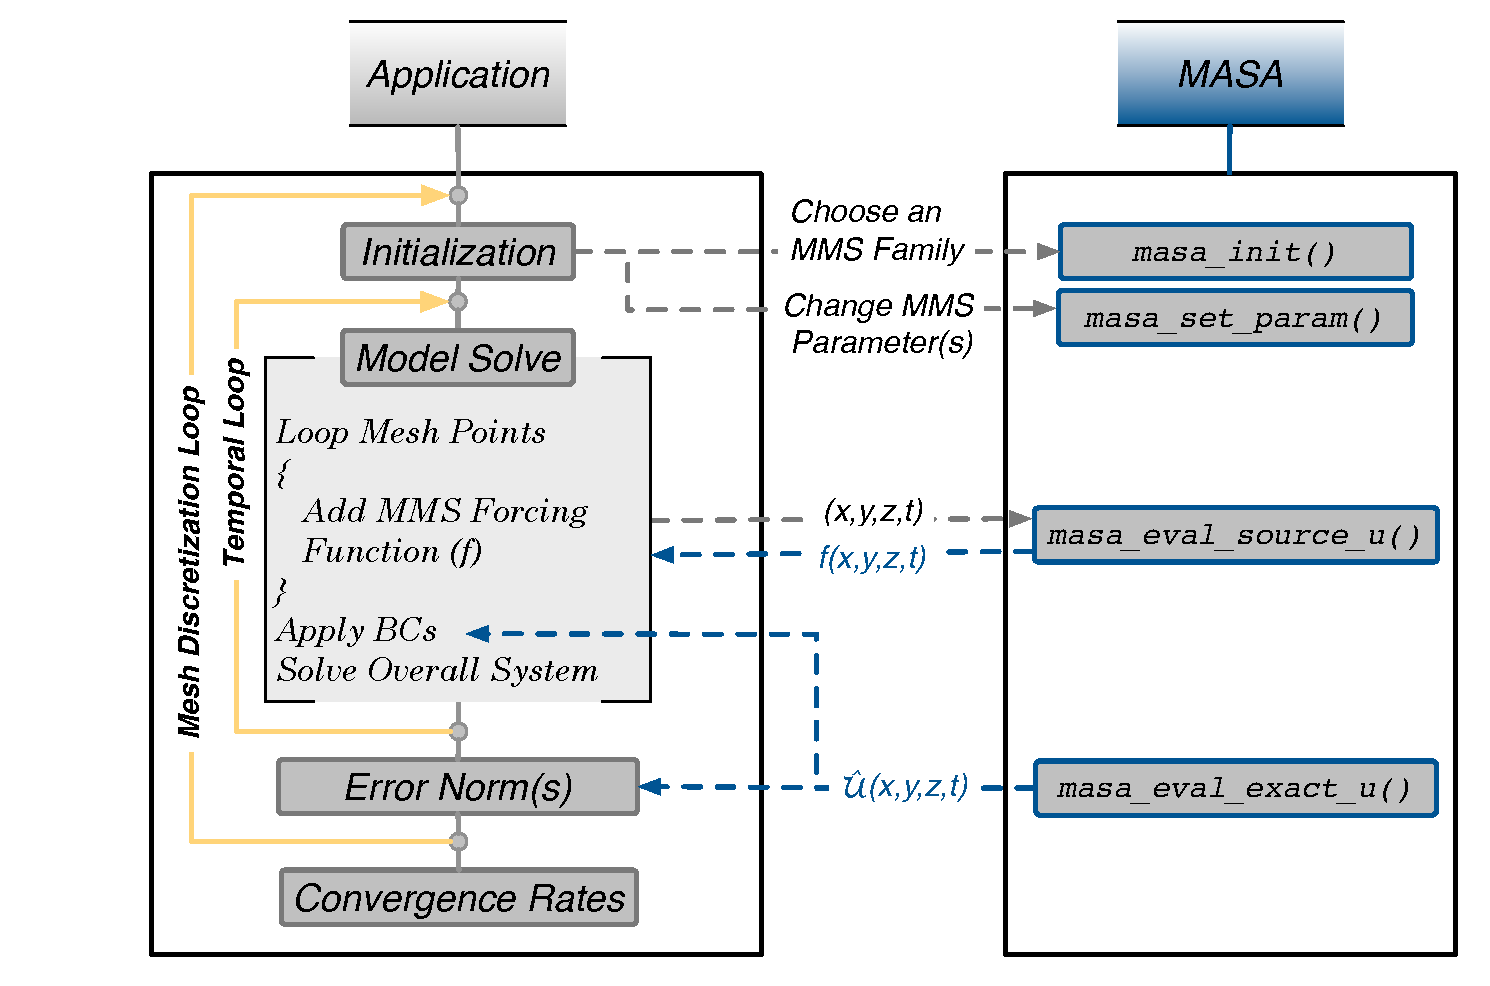
\includegraphics[width=.8\linewidth]{masa_overview} \\
  \end{center}
\end{frame}


\begin{frame}[fragile]
  \frametitle{General Program Flow (a C example)}
{\tiny
%  \begin{center}
  \begin{verbatim}
int main(int argc, char *argv[])
{
  int n;
  double length;
  pstruct model;                /* primary model data structure */

  /* Parse command-line */

  if(argc < 2)
    {
      printf("\nUsage: laplacian [num_pts] [length]\n\n");
      printf("where \"num_pts\" is the desired number of mesh points and \n");
      printf("\"length\" is the physical length-scale dimension in one direction\n\n");
      
      exit(1);
    }
  else
    {
      n      = atoi(argv[1]);
      length = (double) atof(argv[2]);
    }

  /* Problem Initialization */

  problem_initialize (n,length,&model);
  assemble_matrix    (1,&model);
  init_masa          (&model);
  apply_bcs          (&model);

  .....
\end{verbatim}
%  \end{center}
}  
\end{frame}

\begin{frame}[fragile]
  \frametitle{General Program Flow (a C example, continued)}
{\tiny
  \begin{verbatim}

  /* Solve linear system */

  solve_gauss       (&model);

  /* Compute Error */

  printf("\n** Error Analysis\n");
  printf("   --> npts     = %i\n",model.npts);
  printf("   --> h        = %12.5e\n",model.h);
  printf("   --> l2 error = %12.5e\n",compute_l2_error(&model));

  return 0;

}
\end{verbatim}
}  
\end{frame}


%% more code foo
\begin{frame}[fragile]
  \frametitle{Example Model Data Structure}
{\tiny
  \begin{verbatim}

typedef struct pstruct {
  double  *phi;                 /*!< solution variable                    */
  double  *rhs;                 /*!< right-hand side forcing function     */
  double **A;                   /*!< linear system matrix                 */
  double   h;                   /*!< mesh sizing                          */
  int      n;                   /*!< problem size                         */
  int      npts;                /*!< number of points in single direction */
  int      pad;                 /*!< pad dimension for ghost points       */
} pstruct;

\end{verbatim}
}  
\end{frame}

%===============================================================================
% slide where we show an example of just that, using Karls plot
%===============================================================================
\begin{frame}
  \frametitle{Example Results: What we're hoping for}
  2nd Order Central Finite-difference Scheme

\begin{center}
\begin{columns}[c]
\begin{column}{6cm}
    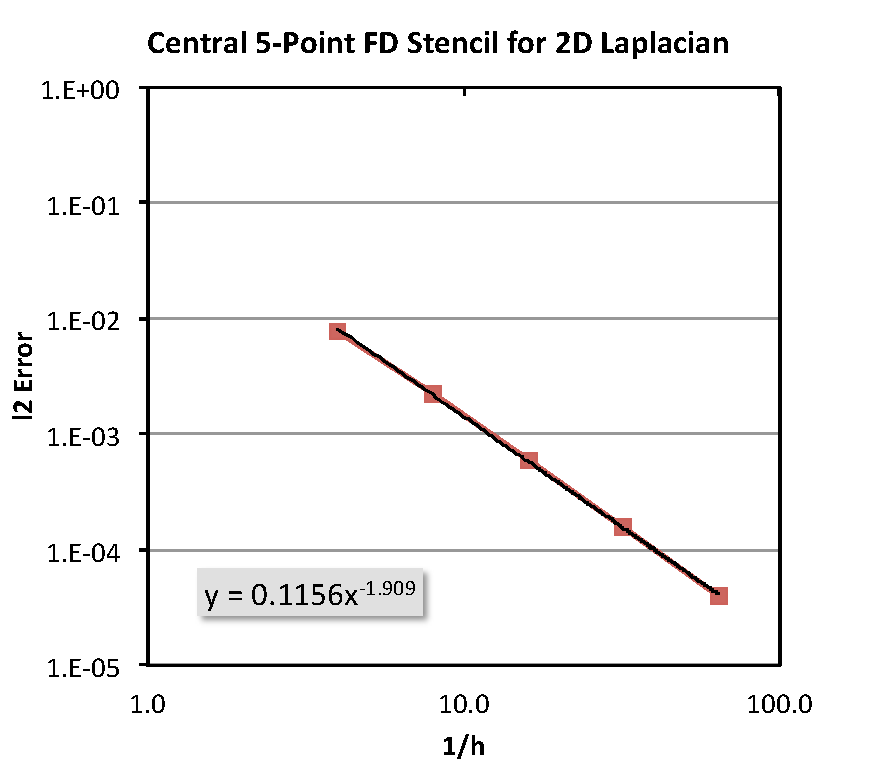
\includegraphics[width=0.95\linewidth]{laplace_central_diff1}
\end{column}
\begin{column}{6cm}
    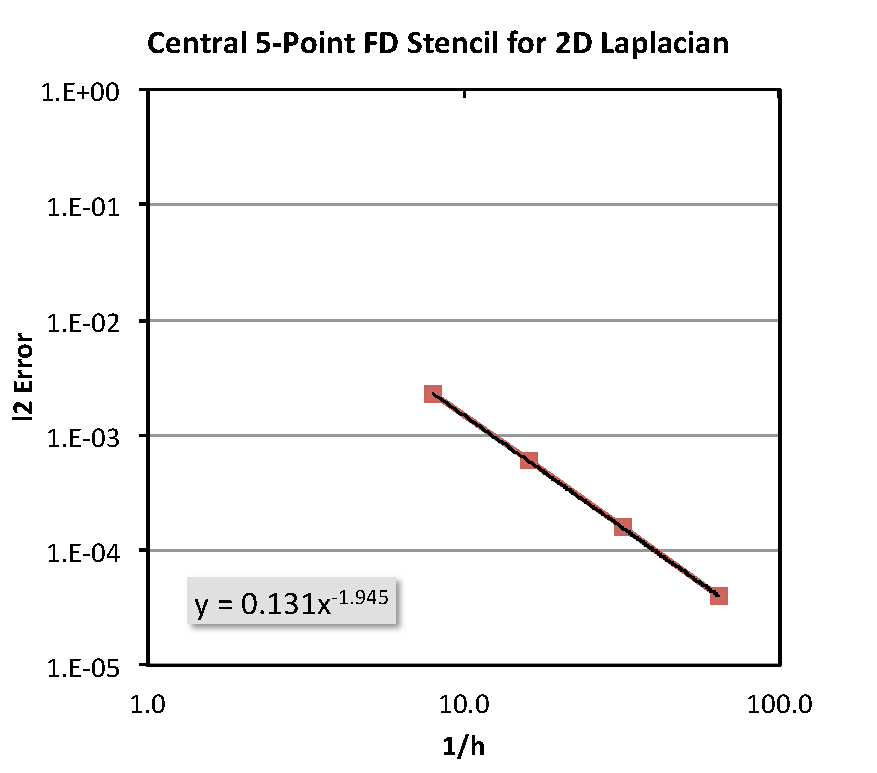
\includegraphics[width=0.95\linewidth]{laplace_central_diff2}
\end{column}
\end{columns}
\begin{itemize}
\item Example results for $\text{npts} = 5,9,17,33,65$, $\text{length} = 1.0$
\end{itemize}
  \end{center}
  
\end{frame}

%===============================================================================
% NEW SLIDE: finis
%===============================================================================
\begin{frame}[fragile]
\frametitle{MASA PDE Examples}

\begin{block}{Source Terms: Euler}
\begin{semiverbatim}
\footnotesize

\comment{// Gas state}
\type{ADScalar} \var{T}  = \var{P} / \var{RHO} / \var{R};
\type{ADScalar} \var{E}  = \data{1.} / (\var{Gamma}-\data{1.}) * \var{P} / \var{RHO};
\type{ADScalar} \var{ET} = \var{E} + \data{.5} * \var{U}.\func{dot}(\var{U});

\comment{// Mass, momentum and energy}
\type{Scalar}   \var{Q_rho}   = \func{raw_value}(\func{divergence}(\var{RHO}*\var{U}));
\type{RawArray} \var{Q_rho_u} = \func{raw_value}(\func{divergence}(\var{RHO}*\var{U}.\func{outerproduct}(\var{U})) +
                   \var{P}.\func{derivatives}());
 \type{Scalar}  \var{Q_rho_e} = \func{raw_value}(\func{divergence}((\var{RHO}*\var{ET}+\var{P})*\var{U}));

\end{semiverbatim}
\end{block}
 {\bf check out tests/ad\_euler.cpp}
\end{frame}

%===============================================================================
% NEW SLIDE: finis
%===============================================================================
\begin{frame}
  \frametitle{}
  \begin{block}{}
    \center{Thank you for your attention.} \\
    \center{Let's start coding!!!}
  \end{block}
\end{frame}

% %===============================================================================
% % goals of workshop
% %===============================================================================
% \begin{frame}
%   \frametitle{Workshop}

%   \begin{block}{Goals}
%     \begin{itemize} 
%     \item Walk you through the process of code verification
%     \item Build/install MASA
%     \item Do a grid-refinement study for solution verification
%     \item Write some code to have a little fun - do something simple
%       and use MASA
%     \end{itemize}    
%   \end{block}

% \end{frame}

% %===============================================================================
% % refresher
% %===============================================================================
% \begin{frame}
%   \frametitle{Problem: Solve 2D Laplacian using Finite-Differencing}
%   \begin{columns}[c]
%     \begin{column}{5cm}

%       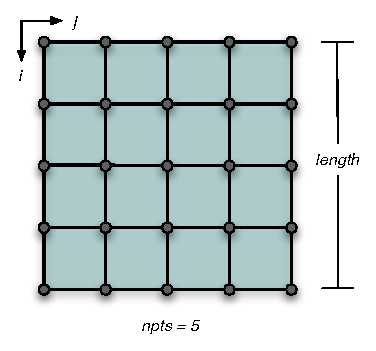
\includegraphics[width=1\linewidth]{domain}

%     \end{column}
    
%     \begin{column}{6.5cm}
      
%       \begin{block}{Recall:}
%         \begin{itemize} 

%           \item Laplace's Equation in 2D:
%           \begin{equation}
%             \nonumber     
%             \frac{\partial^2 \phi}{\partial x^2} + \frac{\partial^2 \phi}{\partial y^2} = 0
%           \end{equation}

% 	  \item For the verification exercise, we will replace the RHS
% 	    above with a forcing function $f(x,y)$ that we get from
% 	    MASA
%           \begin{equation}
%             \nonumber     
%             \frac{\partial^2 \phi}{\partial x^2} + \frac{\partial^2
% 	      \phi}{\partial y^2} = f(x,y)
% 	    \end{equation}
          
%           % nick: not sure about this here, do we want to show mms?
%           % seems less useful to remind them about the source term
% %%           \item Our manufactured solution is:
% %%           \begin{equation}
% %%             \begin{split}
% %%               \nonumber
% %%               \phi(x,y) &= (\textcolor{blue}{Ly}-y)^2 (\textcolor{blue}{Ly}+y)^2 \\ 
% %%               &+ (\textcolor{red}{Lx}-x)^2 (\textcolor{red}{Lx}+x)^2
% %%             \end{split}
% %%           \end{equation}          
% %%           \item By default, \textcolor{blue}{Ly}$=0.82$ and \textcolor{red}{Lx}$=1.4$

%         \end{itemize}    
%       \end{block}
      
%     \end{column}
%   \end{columns}

% %%   % karl: can you check that this is the differencing scheme you intended?
% %%   Solve using forward difference:
% %%   \begin{equation}
% %%     \nonumber     
% %%     \phi_i'' \approx \frac{\phi_{i+2} - 2\phi_{i+1} + \phi_{i}}{h^2} + O(h^2)
% %%   \end{equation}
  
% \end{frame}

% %===============================================================================
% % add slide about laplace equation solution here
% %===============================================================================

% \begin{frame}
%   \frametitle{Manufactured solution to Laplace's Equation}
  
%   Laplace's Equation:
%   \begin{equation}
%       \nonumber      
%     \nabla^2 \phi = 0
%   \end{equation}
%   In two dimensions:
%   \begin{equation}
%       \nonumber      
%     \frac{\partial^2 \phi}{\partial x^2} + \frac{\partial^2 \phi}{\partial y^2} = 0
%   \end{equation}
%   \newline
%   \newline
%   ``Manufacture'' a solution, with two constants:
%   \begin{equation}
%       \nonumber
%     \phi(x,y) = (\textcolor{red}{Ly}-y)^2 (\textcolor{red}{Ly}+y)^2 + (\textcolor{red}{Lx}-x)^2 (\textcolor{red}{Lx}+x)^2
%   \end{equation}  

% \end{frame}


% \begin{frame}
%   \frametitle{Finite-difference Scheme}
%     \begin{block}{Method}
%       \begin{itemize} 
% 	\item Let us use a simple FD approximation for the Laplacian
%         \item Assume a constant spacing mesh for convenience
%         \item Central-differencing 
% 	  \begin{equation}
% 	    \nonumber     
% 	    \nabla^{2}{\phi}_{i,j} \approx \frac{\phi_{i+1,j} -
% 	      2\phi_{i,j} + \phi_{i-1,j}}{h^2} + 
% 	    \frac{\phi_{i,j+1} -
% 	      2\phi_{i,j} + \phi_{i,j-1}}{h^2} + O(h^2)
% 	  \end{equation}
% 	  \item Use this formula to build the coefficient entries into
% 	    a linear system $Ax=b$.  
% 	  \item The size of the linear system is the number of solution
% 	    points. Since we are on a square domain,  $N = npts*npts$
% 	  \item You may find it convenient to use a mapping
% 	    from a 2D index $\phi_{i,j}$ to a 1D index for the
% 	    solution vector of your linear system, $\phi_{\text{index}}$
% 	  \begin{equation}
% 	    \nonumber     
% 	    index = j+(i*npts);
% 	    \end{equation}
%       \end{itemize}
%     \end{block}
% \end{frame}


% \begin{frame}
%   \frametitle{Finite-difference Scheme}
%     \begin{block}{Boundary Conditions}
%       \begin{itemize} 
%           \item The 5-point FD stencil is incomplete on the boundaries of
% 	    our square domain 
% 	  \item We need to apply constraints to matrix
% 	    $A$ to enforce the Dirchlet conditions on the boundaries
% 	  \item Simplest method to enforce BCs:
% 	    \begin{itemize} 
% 	      \item zero out all matrix entries on the
% 		row associated with boundary point, $\phi_i$
% 	    \item set the
% 	      diagonal $A(i,i)$ = 1.0
% 	      \item Set the RHS function to the
% 		desired solution $f_i = \phi_{\text{exact}}$
% 		\end{itemize}
%       \end{itemize}
%     \end{block}
% \end{frame}

% \begin{frame}[fragile]
%   \frametitle{Finite-difference Scheme}
%     \begin{block}{Boundary Conditions}
%       \begin{itemize} 
%           \item Let's look at form of system matrix $A^*$ after BCs have
% 	    been applied for $npts=3$ (note $A=\frac{1}{h^2}A^*$):
% {\tiny
% \begin{verbatim}


%      j =     0      1      2      3      4      5      6      7      8 

% i =  0:   1.00   0.00   0.00   0.00   0.00   0.00   0.00   0.00   0.00 
% i =  1:   0.00   1.00   0.00   0.00   0.00   0.00   0.00   0.00   0.00 
% i =  2:   0.00   0.00   1.00   0.00   0.00   0.00   0.00   0.00   0.00 
% i =  3:   0.00   0.00   0.00   1.00   0.00   0.00   0.00   0.00   0.00 
% i =  4:   0.00   1.00   0.00   1.00  -4.00   1.00   0.00   1.00   0.00 
% i =  5:   0.00   0.00   0.00   0.00   0.00   1.00   0.00   0.00   0.00 
% i =  6:   0.00   0.00   0.00   0.00   0.00   0.00   1.00   0.00   0.00 
% i =  7:   0.00   0.00   0.00   0.00   0.00   0.00   0.00   1.00   0.00 
% i =  8:   0.00   0.00   0.00   0.00   0.00   0.00   0.00   0.00   1.00 


% \end{verbatim}
% }
% \item In this case, we only have {\em one} active interior solution point
%       \end{itemize}
%     \end{block}
% \end{frame}


% %===============================================================================
% % calculate the source term
% %===============================================================================

% \begin{frame}
%   \frametitle{Calculating the Source Term}

%   We insert our manufactured solution back into the governing equations:
%   \begin{equation}
%       \nonumber
%     \frac{\partial^2 ((Lx-x)^2 (Lx+x)^2)}{\partial x^2} + \frac{\partial^2 ((Ly-y)^2 (Ly+y)^2)}{\partial y^2} = 0
%   \end{equation}

%   \begin{equation}
%     \begin{split}
%       \nonumber      
%       = & 2(Lx-x)^2 - 8(Lx-x)(Lx+x)+2(Lx+x)^2 \\
%       + & 2(Ly-y)^2 - 8(Ly-y)(Ly+y)+2(Ly+y)^2 \\
%       \textcolor{red}{\neq} & \textcolor{red}{0}
%     \end{split}
%   \end{equation}
%   This does not satisfy Laplace's Equation!
%   \newline
%   \newline
%   \begin{block}{}
%     To balance the equation, add the residual to the RHS as a source term. 
%   \end{block}
% \end{frame}

% %===============================================================================
% % back to laplace: we have a solution, now what do we do with it?
% %===============================================================================
% \begin{frame}
%   \frametitle{Example Verification Use Case}
%   \begin{block}{}
%     To solve Laplace's Equation numerically, we need a discretization scheme.
%   \end{block}
%   Let's use a 2nd order finite central difference:
%   \begin{equation}
%       \nonumber      
%     \phi_i'' \approx \frac{\phi_{i+1} - 2\phi_{i} + \phi_{i-1}}{h^2} + O(h^2)
%   \end{equation}
%   This requires solving the implicit system of equations: 
%   \begin{equation}
%       \nonumber      
%       A \vec \phi = \textcolor{red}{f}
%   \end{equation}
%    You can use your favorite linear solver (e.g. PETSc) to solve the
%    system.
%  %, or we'll provide a simple (slow) Gauss-Seidel iterative example.
% %  We will use a conjugate gradient solver to invert the matrix A.

% \end{frame}

% %===============================================================================
% % application linkage
% %===============================================================================
% \begin{frame}
%   \frametitle{General Verification Approach Using MMS and MASA}
%   \begin{center}
%     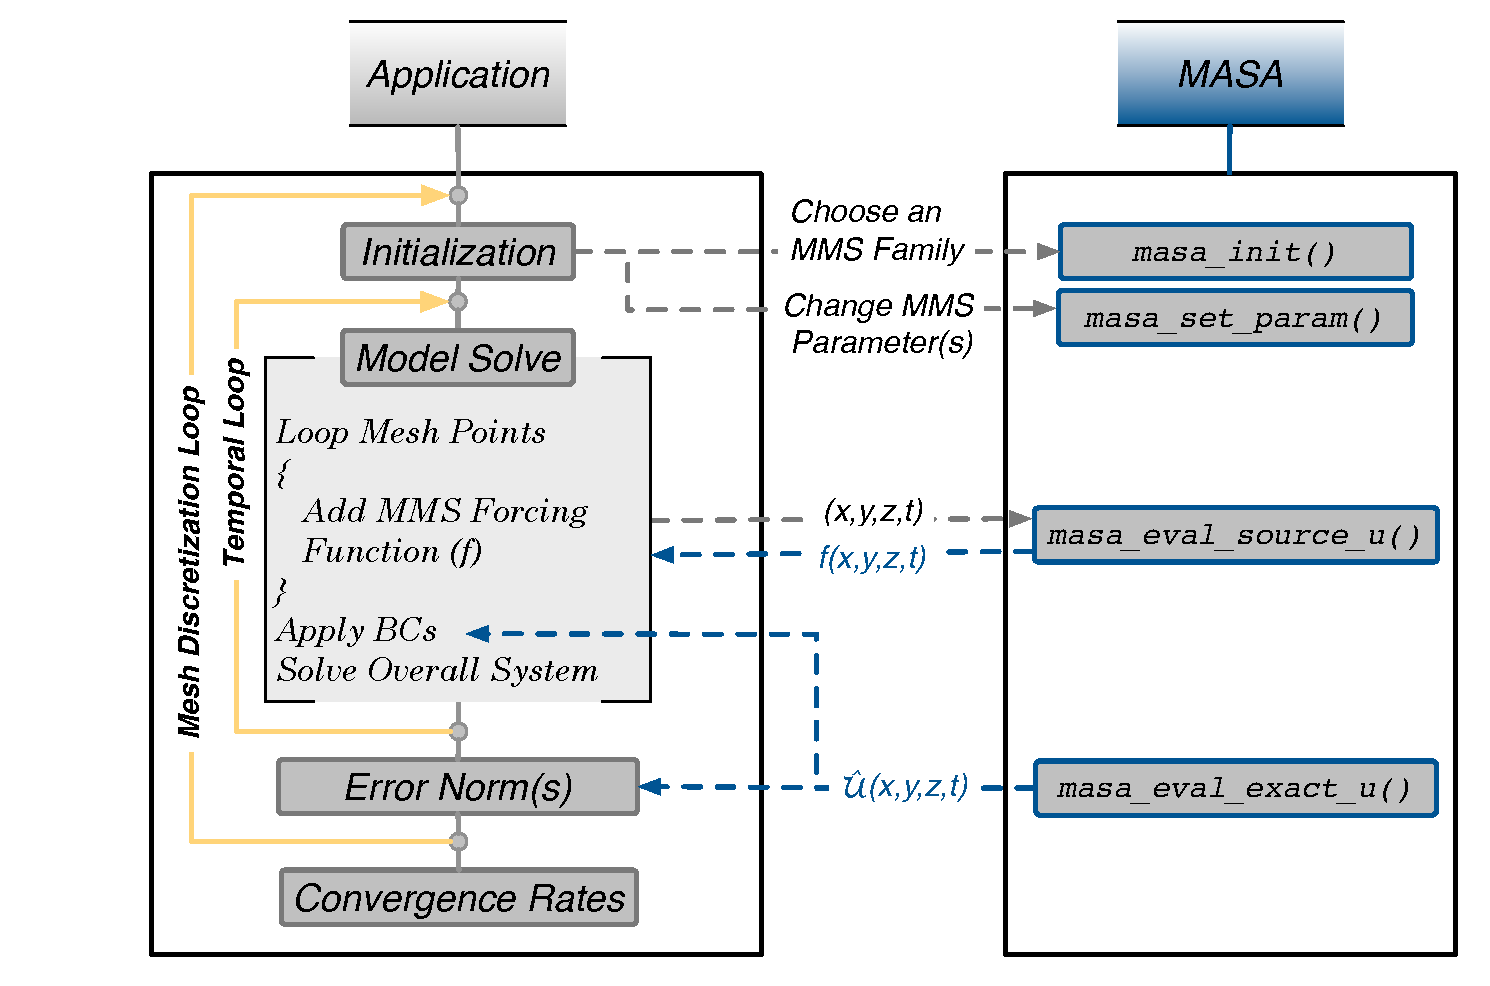
\includegraphics[width=.8\linewidth]{masa_overview} \\
%   \end{center}
% \end{frame}

% %===============================================================================
% % back to laplace: we have a solution, now what do we do with it?
% %===============================================================================

%  \begin{frame}
%    \frametitle{Problem: Solve 2D Laplacian using Finite-Differencing}

%    \begin{block}{Outline}
%      \begin{itemize} 
%      \item {\em Goal:} Write a program in C/C++, F90
%      \item {\em Inputs}: 
%        \begin{itemize}
% 	 \item \# of points in one direction ({\em npts})
% 	 \item the physical dimension of one side ($L_x$, $L_y$)
%        \end{itemize}
%      \item {\em Output}: $l_2$ error between your numerical solution
%        and an exact solution derived from a manufactured solution
%        \begin{equation}
%          \nonumber
%          l_2 = \sqrt{ \frac{\sum_{i=1}^{\text{\tiny N}} (\phi_i-\phi_i^{\text{\tiny exact}})^2}N}
%        \end{equation}
%      \item {\em Runs}: Run your snazzy code for $\text{npts} =
%        5,9,17,\text{and } 33$ and plot $l_2$ norm as a function of $1/h$ where
%        $h=\text{length}/(\text{npts}-1)$
       
%      \end{itemize}    
%    \end{block}

%  \end{frame}

% %% %===============================================================================
% %% % fix bug
% %% %===============================================================================
%  \begin{frame}
%    \frametitle{This Process Finds Bugs}
%       \begin{center}
%         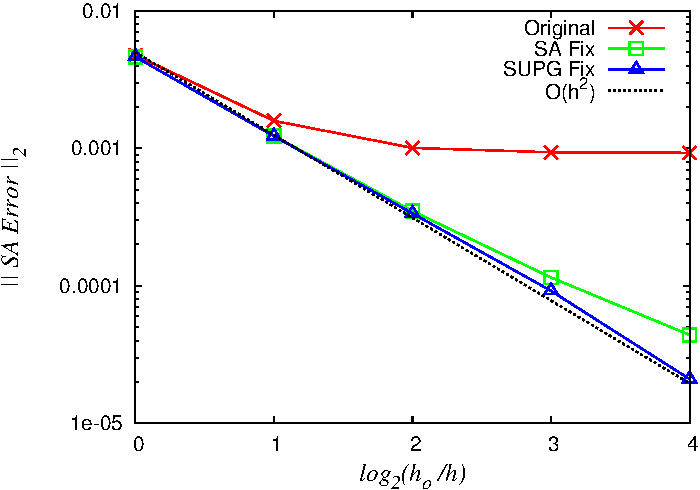
\includegraphics[scale=.8]{mms_grid_convergence.pdf} \\
%       \end{center}

%  \end{frame}
	   
% % Nick to do
% \begin{frame}
%   \frametitle{Installing MASA locally}
%   \begin{block}{Steps for Building MASA:}
%     \begin{itemize}
%       \item Grab latest tarball (https://red.ices.utexas.edu/attachments/download/1352/masa-0.40.2.tar.gz)
%         % bit of a mouthful but thats how it is
%         % https://red.ices.utexas.edu/projects/software/files
%       \item Untar: tar xvfz masa-0.40.2.tar.gz 
%       \item Configure: ./configure --prefix=\$HOME/masa % what about compilers here?
%       \item Compile: make -j 2
%       \item Test: make check
%       \item Install locally: make install
%       \item To generate documenations: make docs 
% 	\begin{itemize}
% 	  \item Can then point a broswer to docs/html/index.html
% 	\end{itemize}
%     \end{itemize}
%    \end{block}

% \end{frame}

% \begin{frame}[fragile]
%   \frametitle{Linking to your installed MASA}
%   \begin{block}{Linking against your local build}
%     \begin{itemize} 

%       \item {\bf C}: Assuming your code is named laplacian.c and you
%       installed masa into \$HOME/masa: 
% {\tiny
% \begin{verbatim}

% gcc -I$HOME/masa/include laplacian.c -L$HOME/masa/lib -lmasa

% \end{verbatim}
% }
      
%       \item {\bf F90}: Assuming your code is named laplacian.f90 
% {\tiny
% \begin{verbatim}

% gfortran -I$HOME/masa/lib laplacian.f90 -L$HOME/masa/lib -lmasa -lfmasa

% \end{verbatim}
% }
%       \end{itemize}
%     \end{block}
% \end{frame}

% %===============================================================================
% % refresher
% %===============================================================================
% \begin{frame}
%   \frametitle{Problem: Solve 2D Laplacian using Finite-Differencing}
%   \begin{columns}[c]
%     \begin{column}{5cm}

%       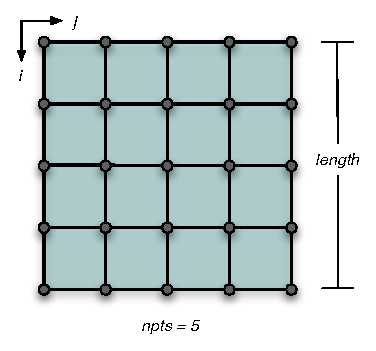
\includegraphics[width=1\linewidth]{domain}

%     \end{column}
    
%     \begin{column}{6.5cm}
      
%       \begin{block}{Recall:}
%         \begin{itemize} 

%           \item Laplace's Equation in 2D:
%           \begin{equation}
%             \nonumber     
%             \frac{\partial^2 \phi}{\partial x^2} + \frac{\partial^2 \phi}{\partial y^2} = 0
%           \end{equation}

% 	  \item For the verification exercise, we will replace the RHS
% 	    above with a forcing function $f(x,y)$ that we get from
% 	    MASA
%           \begin{equation}
%             \nonumber     
%             \frac{\partial^2 \phi}{\partial x^2} + \frac{\partial^2
% 	      \phi}{\partial y^2} = f(x,y)
% 	    \end{equation}
          
%         \end{itemize}    
%       \end{block}
      
%     \end{column}
%   \end{columns}

% \end{frame}

% \begin{frame}
%   \frametitle{Finite-difference Scheme}
%     \begin{block}{Method}
%       \begin{itemize} 
% 	\item Let us use a simple FD approximation for the Laplacian
%         \item Assume a constant spacing mesh for convenience
%         \item Central-differencing 
% 	  \begin{equation}
% 	    \nonumber     
% 	    \nabla^{2}{\phi}_{i,j} \approx \frac{\phi_{i+1,j} -
% 	      2\phi_{i,j} + \phi_{i-1,j}}{h^2} + 
% 	    \frac{\phi_{i,j+1} -
% 	      2\phi_{i,j} + \phi_{i,j-1}}{h^2} + O(h^2)
% 	  \end{equation}
% 	  \item Use this formula to build the coefficient entries into
% 	    a linear system $Ax=b$.  
% 	  \item The size of the linear system is the number of solution
% 	    points. Since we are on a square domain,  $N = npts*npts$
% 	  \item You may find it convenient to use a mapping
% 	    from a 2D index $\phi_{i,j}$ to a 1D index for the
% 	    solution vector of your linear system, $\phi_{\text{index}}$
% 	  \begin{equation}
% 	    \nonumber     
% 	    index = j+(i*npts);
% 	    \end{equation}
%       \end{itemize}
%     \end{block}
% \end{frame}



% %===============================================================================
% % application linkage
% %===============================================================================
% \begin{frame}[fragile]
% \frametitle{Fortran 90: What you need from MASA}
% {\tiny
% \begin{verbatim}
% program main
%   use masa
%   implicit none

%   dx = real(lx)/real(nx)
%   dy = real(ly)/real(ny);

%   ! initialize the problem
%   call masa_init("laplace example","laplace_2d")

%   ! evaluate source terms (2D)
%   do i=0, nx
%      do j=0, ny
         
%         y = j*dy        
%         x = i*dx
        
%         ! evalulate source term
%         field = masa_eval_2d_source_f   (x,y)

%         ! evaluate analytical term
%         exact_phi = masa_eval_2d_exact_phi (x,y)

%      enddo
%   enddo

% end program main

% \end{verbatim}
% }
% \end{frame}

% %===============================================================================
% % MASA API demo
% %===============================================================================
% \begin{frame}[fragile]
% \frametitle{C: What you need from MASA}
% {\tiny
% \begin{verbatim}
% #include <masa.h>

% int main()
% {
%   err += masa_init("laplace example","laplace_2d");

%   // grab / set parameter values
%   Lx = masa_get_param("Lx");
%   masa_set_param("Ly",42.0);

%   for(int i=0;i<nx;i++)
%     for(int j=0;j<nx;j++)
%       {  
%         x=i*dx;
%         y=j*dy;

%         // source term
%         ffield    = masa_eval_2d_source_f (x,y);

%         // manufactured solution
%         phi_field = masa_eval_2d_exact_phi(x,y);

%        } // finished iterating over space
% } //end program
% \end{verbatim}
% }
% \end{frame}

% %===============================================================================
% % convergence plot
% %===============================================================================
% \begin{frame}
%   \frametitle{Example Results: What we're hoping for}
%   2nd Order Central Finite-difference Scheme

%  \begin{center}
%   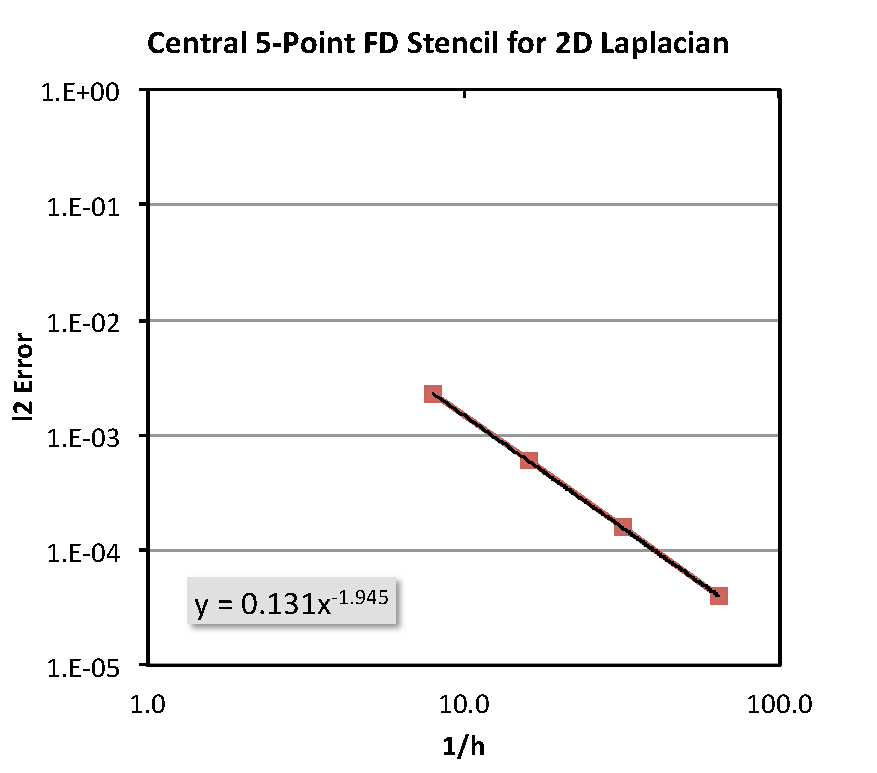
\includegraphics[width=0.7\linewidth]{laplace_central_diff2}
%  \end{center}
  
% \end{frame}

% %===============================================================================
% % conclusions
% %===============================================================================

%  \begin{frame}
%   \frametitle{Conclusions}

%    \begin{block}{}
%     \begin{center}
%      Good Luck!
%     \end{center}
%     \center{Have a well verified day.} \\
%     \center{nick@ices.utexas.edu}
%     \end{block}
%  \end{frame}

\end{document}
